
\chapter{Background}
\label{chap:background}

This chapter explains the \textbf{basic concepts} used throughout the thesis. First, we explain \textbf{neural \acp{lm}}: from the basics of neural networks (§\ref{sec:nns}) and language modeling (§\ref{sec:lm-basics}), up to pretrained (§\ref{sec:plms}) and large language models (§\ref{sec:llms}). Then we move on to \textbf{\ac{d2t} generation}: covering rule-based (§\ref{sec:rule-d2t}) and neural-based systems (§\ref{sec:neural-d2t}), \ac{d2t} datasets (§\ref{sec:datasets}) and evaluation methods (§\ref{sec:evaluation}). We assume that the reader has certain expertise in related areas of \ac{nlp}, although not necessarily in \ac{nlg}. We aim to make the work self-contained by covering all the important concepts, pointing the interested reader to related work for more details.

Besides that, the chapter serves also as an \textbf{overview of the state of the art} in the fields of interest. In particular, the later subsections (\Cref{sec:plms,sec:llms} for neural \acp{lm} and \Cref{sec:neural-d2t,sec:datasets,sec:evaluation} for \ac{d2t} generation) describe the datasets, models, and metrics used for the experiments. As such, the chapter serves as the main point of reference; we will only briefly revisit the most relevant concepts in the respective chapters.


\section{Neural Language Models}
\label{sec:lms}
In this section, we work our way towards neural \acp{lm}: the mathematical foundations of \acp{nn} on which the neural \acp{lm} are built on (\autoref{sec:nns}), the basic ideas of language modeling (\autoref{sec:lm-basics}) and the way \acp{lm} are constructed, trained, and eventually applied in \ac{nlp} (\Cref{sec:plms,sec:llms}).

\subsection{Neural Networks}
\label{sec:nns}
First, we need to build a tool for learning patterns from data\footnote{Until we get to \ac{d2t} generation in \autoref{sec:d2t}, we will use the word ``\textit{data}'' only in its abstract sense, as in ``any inputs we can apply our algorithms to''. We will use the term ``structured data'' whenever it is necessary to make the distinction.}. This tool---which for us will be the \textbf{neural networks}---will later help us with learning patterns about language from large-scale textual data, and in turn with generating text.

Let's say our goal is to predict real-number output $y \in \mathbb{R}$ for the given vector of real numbers $\mathbf{x} = (x_1, \ldots, x_d) \in \mathbb{R}^d$.
% \footnote{We will follow the convention that vectors are denoted with boldface letters ($\mathbf{x}$), and real numbers with plain letters ($x$).} 
We assume that the $\mathbf{x} \rightarrow y$ mapping is not arbitrary (that would leave us with memorizing all the $(\mathbf{x},y)$ pairs), but follows some regularities and underlying patterns that can be learned. This assumption will be naturally satisfied if we consider $(\mathbf{x},y)$ to be representations of real-word data, e.g., documents and their labels.

For learning the underlying pattern between $\mathbf{x}$ and $y$, we will use mathematical models designed to capture the pattern in their parameters. The model estimates the parameters from a limited set of examples called the \textit{training data} and uses the learned parameters to predict the outputs on the \textit{test data}.

\paragraph{Perceptron Algorithm} One of the early mathematical models designed for predicting the outputs based on the inputs is the \emph{perceptron algorithm} (\citealp{rosenblatt1958perceptron}, \citealp[p.~192]{bishop2006pattern}). In this case, we assume the output is a binary class label: $y \in \{-1, 1\}$. The algorithm learns the parameters $\textbf{w} = (w_1, \ldots, w_d) \in \mathbb{R}^d$ and the bias $b \in \mathbb{R}$ describing a linear decision boundary separating the data points according to their class label. The algorithm proceeds as follows:


\begin{enumerate}
    \item The parameters $\textbf{w}$ and $b$ are initialized to small random values or zeros.
    \item For each training example $(\mathbf{x}_i, y_i)$, the algorithm updates the weights and bias to adjust their current estimate towards the ground truth target:
          \begin{align} \label{eq:perceptron1}
              \hat{y}_i  & = \text{sign}(\textbf{w} \cdot \mathbf{x} + b) \\
              \textbf{w} & = \textbf{w} + (y - \hat{y}) \textbf{x}        \\
              b          & = b + y - \hat{y}
          \end{align}
    \item The step (2) is repeated until convergence.
\end{enumerate}

The perceptron algorithm is guaranteed to converge if there exists a hyperplane which separates the data belonging to one class from another, otherwise it will not converge \cite{novikoff1962convergence}.

\paragraph{Multi-layer Perceptron} To overcome the fact that the perceptron is limited to linear decision boundaries, we can use a \textbf{\acl{mlp} (\acs{mlp}}; \citealp[p.~227]{bishop2006pattern}). This mathematical model---also known as a feed-forward neural network---is able to approximate any bounded continuous function \cite{hornik1989multilayer}.

As the name suggests, \ac{mlp} uses multiple perceptron-like units called \textit{neurons}. Analogically to the perceptron (\autoref{eq:perceptron1}), each neuron computes its output $o$ using the rule:
\begin{align}
    o & = f(\mathbf{x}^\top \mathbf{w}  + b),
\end{align}
% \begin{itemize}
where $f: \mathbb{R} \rightarrow \mathbb{R}$ is the \emph{activation function}. Instead of signum, \ac{mlp} uses differentiable non-linear functions, most commonly nowadays \acl{relu} (\acs{relu}; \citealp{nair2010rectified}) or its adapted version \acl{gelu} (\acs{gelu}; \citealp{hendrycks2016gaussian}).

For efficiency, the neurons are organized in layers, which enables formulating the \ac{mlp} computations in terms of matrix multiplication. The $i$-th layer of \ac{mlp} is parametrized with a matrix $\mathbf{W}_i \in \mathbb{R}^{d\times n}$ and a vector of biases $\mathbf{b}_i \in \mathbb{R}^{n}$, processing the \textit{hidden state} $\mathbf{h}_{i-1} \in \mathbb{R}^{d}$ (where we set $\textbf{h}_0 = \textbf{x}$):
\begin{align}
    \mathbf{h}_i & = f(\mathbf{h}_{i-1} \mathbf{W}_i + \mathbf{b}_i).
\end{align}
During training, we aim to minimize the \textit{loss function} describing the gap between the model predictions and the ground truth output. Since all the computations in \ac{mlp} are differentiable, we can use the chain rule to compute how each parameter in the network contributes to the loss. To minimize the loss, we use the \emph{backpropagation} algorithm \cite{kelley1960gradient,rumelhart1986learning}, updating the network parameters in the reverse order of layers. The magnitude of the updates is controlled by the learning rate parameter $\alpha$.

\paragraph{Recurrent Neural Networks} Unlike \acp{mlp}, where the size of the input is fixed, \acp{rnn} allow us to process a sequence of inputs $\mathbf{X} = (\mathbf{x}_1, \ldots, \mathbf{x}_T)$ of arbitrary length. In its vanilla form, the \ac{rnn} computes a sequence of hidden states $\mathbf{H} = (\mathbf{h}^{(0)}, \ldots, \mathbf{h}^{(T)})$ by applying the matrices $\mathbf{W}_h$, $\mathbf{W}_x \in \mathbb{R}^{n\times k}$, and the bias $\mathbf{b} \in \mathbb{R}^{k}$:
\begin{align}
    \mathbf{h}^{(t)} = f(\mathbf{W}_h \mathbf{h}^{(t-1)} + \mathbf{W}_x \mathbf{x}_t + \mathbf{b}).
\end{align}

The hidden state $\mathbf{h}^{(0)} \in \mathbb{R}^k$ is initialized randomly. After the input is processed, $\mathbf{h}^{(T)}$ contains an encoded representation of the sequence.

\acp{rnn} have various shortcomings, including the limited dimensionality of the hidden state and inherently sequential processing. However, they will serve as a stepping stone towards the Transformer architecture described in \autoref{sec:lm-basics}.


\subsection{Language Modeling}
\label{sec:lm-basics}
We will now look into how can we use neural networks to represent and process text.


\paragraph{One-Hot Encoding} Until now, we have assumed that the input to a network is a vector of real numbers. However, a text is a sequence of discrete units such as characters, words, or subwords. To convert these units---called \textit{tokens}---to a numerical representation, we can define a \textit{vocabulary} $V$ which assigns an integer index $i \in \{0, \ldots, |V|-1\}$ to each token.

The naive way to represent each token would be using its integer value. However, this would misleadingly suggest linear dependence between tokens. A better way is to use the index $i$ for constructing a \textit{one-hot} vector $\mathbf{x} \in \{0,1\}^{|V|} $ for each token:
\begin{align}
    x_j = \begin{cases}
        1 & \text{if } i = j, \\
        0 & \text{otherwise}.
    \end{cases}
\end{align}

While this representation is sound, it is quite sparse and does not capture the semantics of individual tokens, requiring that the network learns to represent each token independently.

\paragraph{Word Embeddings} To get a more useful representation of tokens, we may require that tokens with similar meaning are also close in the vector space. Using the distributional theory of meaning \TODO{(Harris, 1954; Firth, 1957)}, we can use the idea that tokens with similar roles also tend to occur in a similar context.

This idea is used in the Word2Vec algorithm \cite{mikolov2013distributed}, which extracts the token representations as the weights of an \ac{mlp} trained either for predicting the tokens in the neighborhood of each token (the \emph{skip-gram} objective) or vice versa, the token itself based on the tokens in its neighborhood (the \emph{continuous bag-of-words} objective). The output of the algorithm is an \textit{embedding matrix} $\mathbf{W}_e \in \mathbb{R}^{|V|\times d}$, which assigns each token a $d$-dimensional \textit{embedding vector} $\mathbf{x} \in \mathbb{R}^{d}$. The objectives are illustrated in \autoref{fig:word2vec}.

Generally, the idea of representing tokens with embedding vectors is employed in neural \acp{lm} described later in this section, where the embedding matrix is the input layer of the model. However, the embedding matrix in neural \acp{lm} is not trained with the aforementioned algorithm, but joinly with the rest of the network.

\begin{figure*}[ht]
    \centering

    \begin{subfigure}{\textwidth}
        \centering
        \begin{subfigure}{0.45\textwidth}
            \centering
            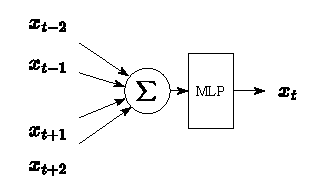
\includegraphics[width=\textwidth]{img/skipgram.pdf}
            \caption{Skip-gram}
            \label{fig:skipgram}
        \end{subfigure}
        \hspace{-20px}
        \begin{subfigure}{0.45\textwidth}
            \centering
            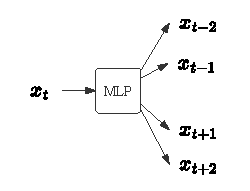
\includegraphics[width=0.75\textwidth]{img/cbow.pdf}
            \caption{Continuous Bag-of-Words}
            \label{fig:cbow}
        \end{subfigure}
    \end{subfigure}
    \caption{The objectives employed by the Word2Vec algorithm \cite{mikolov2013distributed} for learning token embeddings. The algorithm uses a context window of size $k=5$. In the (a) \emph{skip-gram} algorithm, we sum the embeddings of $k-1$ surrounding tokens and predict the original token. In the (b) \emph{continuous bag-of-words} algorithm, we use the original token for predicting the $k-1$ surrounding tokens.}
    \label{fig:word2vec}
\end{figure*}



\paragraph{Tokenization} So far, we have implicitly assumed that we have a way of splitting the text into tokens. Both of the naive approaches---\textit{word-level} and \textit{character-level}---have their own shortcomings. Word-level tokenization will use independent embeddings for morphologically similar words, while character-level tokenization is computationally inefficient.

Subword tokenization algorithms are the middle ground between the two. The goal is to split the text into smaller pieces called \emph{subwords}, so that frequently used words will get their own subword, while less frequent words will be split into multiple subwords.

The algorithm that is frequently used for tokenization in neural \acp{lm} is \textbf{\ac{bpe}}. The \ac{bpe} algorithm starts with the vocabulary of individual bytes, iteratively merging the most frequent tokens and adding them to the vocabulary $V$ until we reach the target vocabulary size. For example, the expression ``Subword tokenization'' could be split into four subwords \texttt{ ['Sub', 'word', '▁token', 'ization']}, the ``\texttt{▁}'' being a special character denoting a preceding space.

\paragraph{Language Models} Having a way to represent text, we can move on to processing and subsequently generating it. A useful formalism in that direction is a \textbf{language model}: a mathematical model that estimates a probability $P(T)$ of a sequence of tokens $T = (t_1, \ldots, t_n)$. For estimating the probability, we can factorize it into a product of conditional probabilities for each token using the chain rule:
\begin{align}
    P(T) = \prod_{i=1}^m P(t_i|t_1, \hdots,t_{m-1}).
\end{align}
Estimating the probability of longer sequences according to this formula is infeasible, as the model would require too many parameters. An \textbf{\emph{n}-gram \ac{lm}} simplifies the product using the assumption that the probability of a token depends only on $n-1$ previous tokens:
\begin{align}
    P(T) = \prod_{i=1}^m P(t_i|t_{i-n+1}, \hdots,t_{i-1}).
\end{align}
The \emph{n}-gram \acp{lm} can be trained by estimating probabilities for individual \emph{n}-grams by tabulating their occurences over a large text corpus. However, because of the simplifying assumption, the \emph{n}-gram \acp{lm} fail to capture long-term dependencies in the text.

\paragraph{Neural \acp{lm}} A neural \ac{lm} is a \acl{lm} that uses a neural network for estimating the text probability. Denoting the parameters of the network by $\theta$ and $\mathbf{X}$ as the sequence of embeddings corresponding to $T$:
\begin{align}
    P(T) = P_\theta(\mathbf{X}).
\end{align}
In contrast with \emph{n}-gram \acp{lm}, the neural network can typically process the whole text, efficiently computing the probability estimates using its hidden states. This makes it suitable for capturing long-term dependencies.


\paragraph{Encoder-Decoder Framework}
We have described a \ac{rnn} (\autoref{sec:nns}) as a neural network that can process the sequence and \emph{encode} its representation in its hidden state.
The idea behind the \textbf{encoder-decoder framework} \cite{sutskever2014sequence,cho2014learning} is that we can \emph{decode} an output sequence with another network using the hidden state of the encoder. With \acp{rnn}, the workflow is the following:

\begin{enumerate}
    \item The \textbf{encoder} encodes the input sentence $\mathbf{X}= (\mathbf{x}_1, \ldots, \mathbf{x}_n)$ into a hidden state $\mathbf{h}_e$ by repeatedly applying a transformation $\mathcal{E}$ in each timestep $i\in(1,n)$:
          \begin{align}
              \mathbf{h}_e^{(i)} = \mathcal{E}(\mathbf{h}_e^{(i-1)}, \mathbf{x}_i).
          \end{align}
    \item The \textbf{decoder} uses $\mathbf{h}_e^{(n)}$ as its initial state $\mathbf{h}_d^{(0)}$ and produces the output sequence  $\mathbf{Y} = (\mathbf{y}_1, \ldots, \mathbf{y}_m)$ by repeatedly applying a transformation $\mathcal{D}$ in each timestep $j\in(1,m)$, using a special \texttt{<BOS>} symbol as $\mathbf{y}_0$:
          \begin{align}
              \mathbf{h}_d^{(j)}, \mathbf{y}_j = \mathcal{D}(\mathbf{h}_d^{(j-1)}, \mathbf{y}_{j-1}).
          \end{align}
\end{enumerate}

\paragraph{Attention Mechanism} The hidden state has a fixed size, which limits the amount of information the network can capture about a sequence. The \textbf{attention mechanism} \cite{bahdanau2015neural} enables the decoder to dynamically extract the information from the encoded sequence. In each step $j$, the decoder computes the weighed average of the encoder hidden states $\{\mathbf{h}_e^{(0)}, \ldots, \mathbf{h}_e^{(n)}\}$ using the attention matrix $\mathbf{W}_a$:
\begin{align}
    \alpha_{ji} & = \operatorname{softmax}(\mathbf{h}_d^{(j)}\mathbf{W}_a \mathbf{h}_e^{(i)}).
\end{align}

The attention vector $\alpha_j$ is used to compute a context vector $c_j$ which is the weighted average of the hidden states of the encoder:
\begin{align}
    \mathbf{c}_j & = \sum_i \alpha_{ji} \mathbf{h}_e^{(i)}
\end{align}
The context vector is used as an additional input for the decoder:
\begin{align}
    \mathbf{h}_d^{(j)}, \mathbf{y}_j = \mathcal{D}(\mathbf{h}_d^{(j-1)}, \mathbf{y}_{j-1}, \mathbf{c}_j).
\end{align}



\paragraph{Transformer Architecture} The Transformer architecture \cite{vaswani2017attention} is a neural network architecture for processing sequences that improves upon \acp{rnn} by enabling efficient parallelization. The architecture is shown in \autoref{fig:transformer}. In its core, the Transformer combines the attention mechanism with \acp{mlp}.

\begin{figure*}[h]
    \centering
    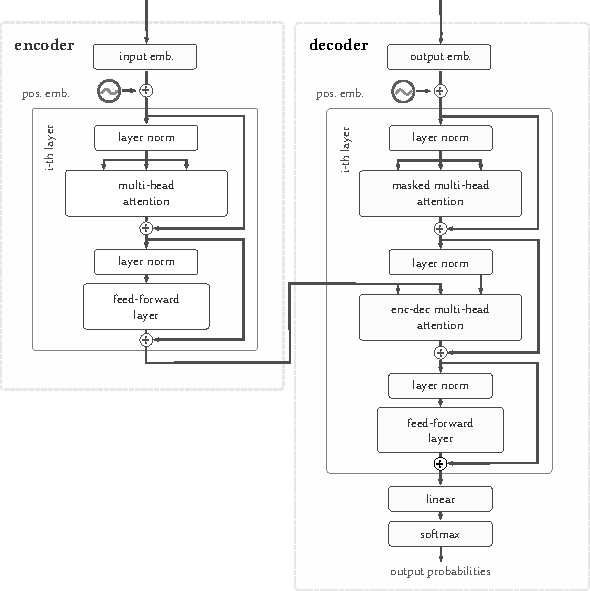
\includegraphics[width=0.9\textwidth]{img/transformer.pdf}
    \caption{A variant of the Transformer architecture. Adapted from \href{https://github.com/bbycroft/llm-viz/blob/main/src/llm/intro-image.svg}{https://github.com/bbycroft/llm-viz}.}
    \label{fig:transformer}
\end{figure*}


\subsection{Pretrained Language Models}
\label{sec:plms}

\paragraph{Encoder Models}

\paragraph{Encoder-Decoder Models}

\paragraph{Decoder Models}

\subsection{Large Language Models}
\label{sec:llms}
\section{Data-to-Text Generation}
\label{sec:d2t}
\subsection{Rule-based Approaches}
\label{sec:rule-d2t}
\subsection{Neural Approaches}
\label{sec:neural-d2t}
\subsection{Datasets}
\label{sec:datasets}
\subsection{Evaluation Metrics}
\label{sec:evaluation}